\section{AMBA Protocol Case Study}\label{amba:sec}

We demonstrate how to synthesize a parameterized implementation of the AMBA AHB,
with guaranteed correctness for any number of masters.
To this end, we translate the LTL specification of the 
AMBA AHB (as found in~\cite{BarbaraThesis}) into a version that is suitable 
for parameterized synthesis in token rings, and address several challenges 
with respect to theoretical applicability and practical feasibility:
\li
\- We show how to localize global input and output signals (those that cannot be assigned to one particular master).
   This is necessary since our approach is based on the replication of components that act only on local information.
\- We extend the cutoff results to fully asynchronous timing model and systems with two process templates.
\- We describe further optimizations that make synthesis feasible,
   in particular based on the insight that the AMBA protocol features three 
   different types of accesses, and the control structures for these accesses 
   can be synthesized step-by-step.
\il

\subsection{Description of the AMBA Protocol} \label{sec:amba}

ARM’s \emph{Advanced Microcontroller Bus Architecture} (AMBA)~\cite{AMBAspec} 
is a communication bus for a number of masters and
clients on a microchip. One of the crucial parts of AMBA is
the \emph{Advanced High-performance Bus} (AHB),
a system bus for the efficient connection of processors, memory, and devices.

For convenience, the input signals are depicted in \textcolor{red}{red} color
and the outputs are \textcolor{blue}{blue}.

The bus arbiter ensures that only one master accesses the bus at any time.
Masters send \hbusreq\ to the arbiter if they want access, and receive
\hgrant\ if they are allowed to access it.
Masters can also ask for different
kinds of \emph{locked transfers} that cannot be interrupted.

The exact arbitration 
protocol for AMBA is not specified. Our goal is to synthesize a protocol 
that guarantees safety and liveness properties. According to the 
specification, any device that is connected to the bus will react to an input 
with a delay of one time step. I.e., we are considering Moore machines. In 
the following, we introduce briefly which signals are used to
realize the arbiter of this bus for masters.

\parbf{Requests and grants}
The identifier of the master which is 
currently active is stored in the $n+1$-bit signal \hmaster[$n$:0], 
with $n$ chosen such that the number of masters fit into $n+1$ bits.
To request the 
bus, master $i$ raises signal \hbusreqi. The arbiter decides who will be 
granted the bus next by raising signal \hgranti. When
the client raises \hready, the bus access starts at the next tick, and there 
is an update \hmaster[$n$:0] := i, where \hgranti\ is currently active.

\parbf{Locks and bursts}
A master can request a locked access by raising both \hbusreqi\ and \hlocki. In this case, 
the master additionally sets \hburst[1:0] to either \ambasignal{single} 
(single cycle access), \hburstfour\ (four cycle burst) or \hincr\ (unspecified 
length burst). For a \hburstfour\ access, the bus is
locked until the client has accepted 4 inputs from the master (each signaled by
raising \hready). In case of a \hincr\ access, the bus is
locked until \hbusreqi\ is lowered. The arbiter raises \hmastlock\ if the bus 
is currently locked.

\parbf{LTL specification}\ak{where $\G \neg g_1 \land g_2$?}
The original natural-language specification~\cite{AMBAspec} has been translated into a formal specification in the GR(1) fragment of LTL before in~\cite{BarbaraThesis,Bloem12,GodhalCH13}.
Figure~\ref{amba:fig:AMBAspec} shows the environment assumptions and system guarantees from~\cite{BarbaraThesis} that serve as the basis for our parameterized specification.
The full specification is 
$ (A1 \land \ldots \land A4) \rightarrow (G1 \land \ldots \land G11)$.
% 
\begin{figure}[t]
  \fbox{%
  \begin{minipage}{\textwidth}
  \[
{\footnotesize
\begin{array}{rrlr}
\multicolumn{3}{l}{\mathrm{Assumptions:}} \\[2pt]
& \always & (\hmastlock \land \hburst = \hincr) \rightarrow \nextt \eventually \neg \hbusreqi[\hmaster] & (A1)\\[3pt]
& \always \eventually & \hready & (A2) \\[3pt]
\forall \mathrm i: & \always & \hlocki \rightarrow \hbusreqi & (A3) \\[3pt]
\forall \mathrm i: & & \neg \hbusreqi \land \neg \hlocki \land \neg \hready & (A4) \\[3pt]
\multicolumn{3}{l}{\mathrm{Guarantees:}} \\[2pt]
& \always & \neg \hready \rightarrow \nextt \neg \hstart & (G1) \\[3pt]
& \always & (\hmastlock \land \hburst = \hincr \land \hstart)\\
& & ~\rightarrow \nextt (\neg \hstart \weakuntil (\neg \hstart \land \hbusreqi[\hmaster])) & (G2) \\[3pt]
& \always & (\hmastlock \land \hburst = \hburstfour \land \hstart \land \hready)\\
& & ~\rightarrow \nextt (\neg \hstart \weakuntil[3] (\neg \hstart \land \hready)) & (G3.1) \\[3pt]
& \always & (\hmastlock \land \hburst = \hburstfour \land \hstart \land \neg \hready)\\
& & ~\rightarrow \nextt (\neg \hstart \weakuntil[4] (\neg \hstart \land \hready)) & (G3.2) \\[3pt]
\forall \mathrm i: & \always & \hready \rightarrow (\hgranti \leftrightarrow \nextt (\hmaster = {\mathrm i})) & (G4)\\[3pt]
& \always & \hready \rightarrow (\hlocked \leftrightarrow \nextt (\hmastlock)) & (G5)\\[3pt]
\forall \mathrm i: & \always & \nextt \neg \hstart \impl \left(
\begin{array}{ll}
 & (\hmaster = {\mathrm i} \leftrightarrow \nextt (\hmaster = {\mathrm i}))\\
\land & (\hmastlock \leftrightarrow \nextt \hmastlock)
\end{array}
 \right) & (G6)\\[3pt]
\forall \mathrm i: & \always & (\hdecide \land \nextt \hgranti) \rightarrow (\hlocki \leftrightarrow \nextt (\hlocked)) & (G7)\\[3pt]

\forall \mathrm i: & \always & \neg \hdecide\ \impl \left(
\begin{array}{ll}
       & \hgranti \leftrightarrow \nextt \hgranti \\
 \land & \hlocked \leftrightarrow \nextt \hlocked
\end{array}
\right) & (G8)\\[3pt]

% \forall \mathrm i: & \always & \neg \hdecide\ \impl \left( (\hgranti \leftrightarrow \nextt \hgranti) \land (\hlocked \leftrightarrow \nextt \hlocked) \right) & (G8)\\[3pt]
\forall \mathrm i: & \always & \hbusreqi \impl \eventually (\neg
\hbusreqi \lor \hmaster = \mathrm i) & (G9)\\[3pt]
\forall \mathrm i\neq 0: & \always & \neg \hgranti \impl (\neg \hgranti \weakuntil \hbusreqi) & (G10.1)\\[3pt]
& \always & (\hdecide \land (\forall \mathrm i: \neg \hbusreqi)) \impl \nextt \hgrant[0] & (G10.2) \\[3pt]
& & \hgrant[0] \land (\forall \mathrm i \neq 0: \neg \hgranti) \land \hmaster = 0 \land \neg \hmastlock \\
& & \land \hdecide \land \hstart & (G11)
\end{array}}\]

  \end{minipage}}
\caption{Specification of the AMBA AHB~\cite{BarbaraThesis}, in the GR(1) fragment of LTL.
  The inputs are:
  \hburst, \hbusreq[i], \hready, and \hlock[i].
  The outputs are:
  \hmastlock, \hmaster, \hstart, \hdecide, \hlocked, and \hgrant[i].}
\label{amba:fig:AMBAspec}
\end{figure}
%

\parbf{Challenges}
The AMBA specification has global inputs and outputs (those are without ``$[i]$''),
distinguishes 0 from non-0 processes (G10.1 and G11),
has the assume-guarantee form $\A(\forall i. A1\land...\land A4 \impl \forall i.G1\land...\land G11)$
(thus not in the prenex-indexed form),
has the process quantification inside a temporal operator in G10.2 $\G(\forall i... \impl ...)$,
and requires a synchronous mode of execution (all processes transit simultaneously).
Thus we cannot apply the cutoff results (Theorem~\ref{tok_rings:thm:cutoffs} on page~\pageref{tok_rings:thm:cutoffs})
for parameterized synthesis.
The next section shows how to handle this.


% We will show how we can use our approach for parameterized synthesis in token 
% rings for synthesizing component implementations for the AMBA AHB 
% specification, such that every component serves the requests of one master, 
% and the composition of an arbitrary number of components is correct by 
% construction. To illustrate our solution, we first review the parameterized 
% synthesis approach, and then mention a number of problems that need to be 
% solved for the AMBA case study.

%\subsection{Additional Definitions}
%

\subsection{Handling the AMBA Specification}\label{amba:sec:handling-amba}

  This section shows how to rewrite the AMBA specification into a form
  admissible to the parameterized synthesis.
  We not only rewrite the specification,
  but also extend the cutoff results~\cite{Emerso03} to the resulting class of specifications.
  Note that the resulting specification is not the same as the original AMBA (but closely resembles it),
  due to constraints of the token-ring architecture.
  (For example, token rings cannot ensure immediate granting of a client,
   because the token has to travel to the corresponding process first.)
  The resulting specification describes a round-robin arbiter
  with different granting schemes and one special process.

%%%%The AMBA specification (Figure~\ref{amba:fig:AMBAspec}) has the form
%%%%$
%%%%(A1 \land \ldots \land A4) \impl (G1 \land \ldots \land G11).
%%%%$
%%%%The specification poses
%%%%the following challenges to existing parameterized synthesis approach~\cite{JB12}
%%%%and cutoff results~\cite{Emerso03,AJKR14}:

\subsubsection{Special 0-process: two process templates $(A,B)$}

  The specification distinguishes between master number 0 and all other masters.
  We support this by synthesizing two different process implementations,
  $A$ for the 0-process and $B$ for non-0 processes:
  the $A$-process serves master 0 and the $B$-processes serve the other masters.
  We denote a token-ring system composed of one $A$ process and $n$ copies of $B$
  using the notation $(A,B)^{(1,n)}$.
  The modified parameterized synthesis problem is to find $(A,B)$ such that
  $\forall n: (A,B)^{(1,n)} \models \Phi$.
  Later we will separate the specification into two parts:
  one will talk about process $A$, another will talk about $B$-processes.

\subsubsection{Localizing global outputs}

  The AMBA specification has global outputs \hmastlock, \hmaster, \hstart, \hdecide, and \hlocked.
  They depend on the global state of the system,
  which is not handled by the work on parameterized model checking of token ring systems~\cite{Emerso03,AJKR14}.
  To overcome this,
  we introduce local versions of the global outputs and build global outputs from them:
  \li
  \- $\hmaster = i$ whenever $\hmasteri$ is high, and 
  \- for every global output $glob$ from $\{\hmastlock, \hstart, \hdecide, \hlocked\}$,
     $glob = \exists{i}.\ \toki \land glob_i$.
  \il
    
  We replace each global output with its local version, e.g., $\hstart$ is replaced by $\hstarti$.
  Note that the limited communication interface (via token passing)
  does not make AMBA specification unrealizable,
  although processes cannot access the value of global outputs when they do not possess the token.
  Intuitively, this is because the token is the shared resource that guarantees mutual exclusion of grants, and therefore the values of these global signals should always be controlled by the process that has the token. In particular, outputs \hdecide\ and \hstart\ are used to decide when to raise a grant and when to start and end a bus access\footnote{The original AMBA specification~\cite{AMBAspec} does not have these signals---they were introduced to simplify the formalization of the specification~\cite{BarbaraThesis}.}, which should only be done when the token is present.
  Similarly, signals \hmastlock\ and \hmaster\ should be controlled by the process that currently controls the bus (and hence has the token). 

  Finally, we mentioned many times that the token should be used to ensure the mutual exclusion of grants.
  Let us explicitly add this requirement into the specification,
  namely we add G12: $\forall i.\,\hgranti \rightarrow \toki$.
  (The original formula contains only an \emph{implicit} mutual exclusion property:
   G4 defines how \hmaster\ is updated by the \hgranti\ signals,
   which can only be satisfied if \hgranti\ are mutually exclusive.)

\subsubsection{Splitting the specification into two \& other small rewritings}

  Once we localized global outputs,
  we can talk about splitting the AMBA specification into two parts.
  At first, each part will be in the assume-guarantee form,
  where the assumptions talk about all the processes (the only $A$ and all $B$),
  but the guarantees will be separated into
  (i) guarantees for the $B$-processes and
  (ii) guarantees for the process $A$.

  After the localization, guarantees G10.1 and G10.2 become:
  \[\begin{array}{rrlr}
  \forall \mathrm i\neq 0\!:\!\!\!\!\! & \always & \neg \hgranti \impl (\neg \hgranti \weakuntil \hbusreqi) & (G10.1)\\[3pt]
  & \always & (\hdecide[0] \land \forall \mathrm i.\neg \hbusreqi) \impl \nextt \hgrant[0] & (G10.2) \\[3pt]
  \end{array}\]
  Thus, G10.1 is used for $B$-processes,
  while G10.2 is used for the process $A$.
  Let us talk more about G10.2, because it has two issues.

  The first issue with G10.2 is that it requires an immediate reaction to a situation when no process receives a bus request. 
  This is unrealizable in token rings,
  because mutual exclusion of the grants requires possession of the token,
  and the token transmission takes time.
  We modify G10.2 to allow the process $A$ to wait for the token and then immediately react:
  $$
  \G
  \big(
  \neg \tok[0] \land \X \tok[0] \land \forall \mathrm i. \neg \hbusreqi
  \impl
  \nextt \hgrant[0]
  \big).
  \footnote{Maybe you expected to see
    $\always \ (\hdecide[0] \land (\forall \mathrm i: \neg \hbusreqi) \land \nextt \tok[0])
    \impl \nextt \hgrant[0])$, 
    but this makes the specification unrealizable due to the token ring requirement 
    $\always (\tok \impl \eventually \send)$: 
    the environment falsifies it by making $\forall \mathrm i: \neg \hbusreqi$ true whenever the process raises $\hdecide$ (and hence the process should continue granting and cannot release the token).
    To regain realizability one could add additional assumptions (something like $\G\F (\hdecide\land\neg\norequests)$). 
    Instead, we decided to change slightly the specification.%
  }
  $$

  The second issue with G10.2 is the quantifier $\forall{i}$ \emph{inside} the temporal operator $\G$
  (such specifications were not studied in parameterized model checking of token rings).
  It requires the process $A$ to know about inputs of all $B$-processes,
  as it needs to react to a situation where \hbusreqi\ is low for every process.
  To get rid of the nesting $\G(\forall i...)$,
  we introduce a new global input $\norequests$,
  and add the assumption $\forall{i}.\G (\hbusreqi \impl \neg \norequests)$.
  Then G10.2 becomes:
  $$
  \G \ 
  (\neg \tok[0] \land \X \tok[0] \land \norequests)
  \impl \X \hgrant[0]).
  $$
  This strengthens the specification,
  because the environment can set $\neg\norequests$
  even when there are no requests.
  This concludes the discussion of G10.2.

  The last asymmetric property is the guarantee G11. We split it into two parts:
  \li
  \- G11.1: $\neg \hgranti \land \neg \hmastlocki$ for $B$-processes and
  \- G11.2: $\tok[0] \impl \hgrant[0] \land \hmaster[0] \land \neg \hmastlock[0]$ (for $A$).
  \il
  % In the general case, if allow index quantifiers inside temporal operators, then parameterized model checking becomes undecidable even for systems with no synchronization at all~\cite[Appendix A]{Igor}.
  % However, for the special case of G10.2 their undecidability proof breaks.\ak{so what?}
  % since G10.2 contains only a single index quantifier inside the topmost $\always$ operator.

\subsubsection{Localizing global inputs}

  The AMBA specification in Figure~\ref{amba:fig:AMBAspec} uses global inputs \hburst,\hready,
  and \norequests\ that we introduced in the previous section.

  First, we introduce local versions $\hburst[i]$, $\hready[i]$, and $\norequests[i]$,
  and add the assumption $\forall i\neq j.\ loc_i = loc_j$ for $loc \in \{\hburst, \hready,\norequests\}$.
  This rewriting does not change the specification.
  The specification becomes
  \begin{align*}
  &\A\Big(\forall{i \neq j}_{i,j \in \{A,B_1,...,B_n\}}. \Phi({i,j}) ~\impl~ \forall{k \in \{B_1,...,B_n\}}. \Psi(k)\Big) ~\land\\
  &\A\Big(\forall{i \neq j}_{i,j \in \{A,B_1,...,B_n\}}. \Phi'({i,j}) ~\impl~ \Psi'(A)\Big),
  \end{align*}
  where each $\Phi(i,j)$ and $\Phi'(i,j)$ talk about propositions of processes $i$ and $j$,
  and $\Psi(k)$ and $\Psi'(A)$ talk about propositions of process $k$ and $A$ respectively.
  Note that $\Psi \neq \Psi'$ because we split the guarantees for $B$-processes and the process $A$
  (the assumptions also slightly differ, so we use $\Phi$ and $\Phi'$).
  Now the specification does neither have global inputs nor global outputs.

  Second, we drop the newly introduced assumptions.
  This means that the original global inputs $\hburst$, $\hready$, and $\norequests$ may have different values for different processes,
  i.e., they are not ``global'' anymore.
  This strengthens the specification,
  because dropping the assumptions enables more environment behaviors (and the formula is universal $\A(...)$).
  The resulting specification becomes
  \begin{equation}\label{eq:amba:assume-guarantee-spec}
  \begin{aligned}
  &\A\big(\forall{i \in \{A,B_1,...,B_n\}}. \Phi(i) ~\impl~ \forall{j \in \{B_1,...,B_n\}}. \Psi(j)\big) ~\land\\
  &\A\big(\forall{i \in \{A,B_1,...,B_n\}}. \Phi'(i) ~\impl~ \Psi'(A)\big).
  \end{aligned}
  \end{equation}
  Figures~\ref{fig:AMBASpecNewI}~and~\ref{fig:AMBASpecNew0} define $\Phi$, $\Psi$, $\Phi'$, and $\Psi'$.
  We stress that $\Phi(i)$ and $\Phi'(i)$
  has to be conjoined over all $B$-processes \emph{and} the process $A$ to form the assumptions.

  \begin{figure}%[t]
    \fbox{%
    \begin{minipage}{\textwidth}
    \[
{
\footnotesize
\begin{array}{llrlr}
% \forall \mathrm i: & \always & (\hmastlocki \land (\hburst = \hincr) \land \hmasteri) \rightarrow \nextt \eventually \neg \hbusreqi & (A1)\\[3pt]
\multicolumn{4}{l}{\text{Assumptions $\Phi(i)$:}} \\[2pt]
%  & \always\eventually & \hready & (A2) \\[3pt]
%& & \multicolumn{1}{l}{\hready \textit{ is global}} \\[3pt]
% \hready \ \ \text{is global} & & & \\[3pt]
& & \G & ((\hmastlocki \land (\hbursti = \hincr) \land \hmasteri) \rightarrow \nextt \eventually \neg \hbusreqi) & (A1) \\[3pt]
& & \G\F & \hreadyi & (A2) \\[3pt]
& & \G & \hlocki \rightarrow \hbusreqi & (A3) \\[3pt]
& & & \neg \hbusreqi \land \neg \hlocki \land \neg \hreadyi & (A4) \\[5pt]
%& & \always & \eventually \toki & (A5) \\[3pt]

\multicolumn{4}{l}{\text{Guarantees $\Psi(i)$:}} \\[3pt]
& & \always & \neg \hreadyi \rightarrow \nextt \neg \hstarti & (G1) \\[3pt]
& & \always & (\hmastlocki \land \hbursti = \hincr \land \hstarti)\\
& & & ~\rightarrow \nextt (\neg \hstarti \weakuntil (\neg \hstarti \land \hbusreqi)) & (G2) \\[3pt]
& & \always & (\hmastlocki \land \hbursti = \hburstfour \land \hstarti \land \hreadyi)\\
& & & ~\rightarrow \nextt (\neg \hstarti \weakuntil[3] (\neg \hstarti \land \hreadyi)) & (G3.1) \\[3pt]
& & \always & (\hmastlocki \land \hbursti = \hburstfour \land \hstarti \land \neg \hreadyi)\\
& & & ~\rightarrow \nextt (\neg \hstarti \weakuntil[4] (\neg \hstarti \land \hreadyi)) & (G3.2) \\[3pt]
& & \always & \hreadyi \rightarrow (\hgranti \leftrightarrow \nextt \hmasteri) & (G4)\\[3pt]
& & \always & \hreadyi \rightarrow (\hlockedi \leftrightarrow \nextt \hmastlocki) & (G5)\\[3pt]
& & \always & \nextt \neg \hstarti \impl \left(
\begin{array}{ll}
 & \hmasteri \leftrightarrow \nextt \hmasteri\\
\land & \hmastlocki \leftrightarrow \nextt \hmastlocki
\end{array}
 \right) & (G6)\\[3pt]
& & \always & (\hdecidei \land \nextt \hgranti) \rightarrow (\hlocki \leftrightarrow \nextt \hlockedi) & (G7)\\[3pt]

& & \always & \neg \hdecidei\ \impl \left(
\begin{array}{ll}
       & \hgranti \leftrightarrow \nextt \hgranti \\
 \land & \hlockedi \leftrightarrow \nextt \hlockedi
\end{array}
\right) & (G8)\\[3pt]




& & \always & \hbusreqi \impl \eventually (\neg
\hbusreqi \lor \hmasteri) & (G9)\\[3pt]
& & \always & \neg \hgranti \impl (\neg \hgranti \weakuntil \hbusreqi) & (G10.1)\\[3pt]
% \forall \mathrm i: & \always & (\hdecidei \land (\forall \mathrm i: \neg \hbusreqi)) \impl \nextt \hgrant[0] & (G10.2) \\[3pt]
& & & \neg \hgranti \land \neg \hmastlocki & (G11.1) \\[3pt]
& & \always & \hgranti \impl \toki & (G12)
\end{array}}\]

    \end{minipage}
    }
    \caption{Parameterized AMBA specification for $B$-processes:
      assumptions $\Phi(i)$ and guarantees $\Psi(i)$.
      G10.2 is omitted, since it is only needed for the process $A$.%
    }
    \label{fig:AMBASpecNewI}
  \end{figure}
  \begin{figure}%[t]
    \fbox{%
    \begin{minipage}{\textwidth}
    \[ 
{\footnotesize
\begin{array}{rllr}


\multicolumn{4}{l}{\text{Assumptions $\Phi'(i)$:}}\\[2pt]
%\text{Assumptions $\Phi(i)$:} 
& \textit{~~~~as before: } & A1, A2, A3, A4 \\[3pt]

& \textit{~~~~new: } & \always~~ \hbusreqi \impl \neg \norequestsi & (A6)\\ [5pt]

\multicolumn{4}{l}{\text{Guarantees $\Psi'(0)$:}}\\[2pt]
& \textit{~~~~as before: } &  G1, G2, G3, G4, G5, G6, G7, G8, G9, G12 ~~ (\text{where $i=0$}) &  \\[3pt]

& \textit{~~~~removed: } & G10.1, G11.1\\[3pt]

& \textit{~~~~modified:} & \always (\norequests[0] \land \neg \tok[0] \land \nextt \tok[0])
  \impl
  \X \hgrant[0])& (G10.2) \\[3pt]

& \textit{~~~~modified:}& \tok[0]\impl\hgrant[0]\land\hmaster[0]\land\neg \hmastlock[0]  & (G11.2)

\end{array}
}
\]

    \end{minipage}}
    \caption{Parameterized AMBA specification for the process $A$:
      modifications wrt.\ Figure~\ref{fig:AMBASpecNewI}.
      The index $0$ denotes the process $A$.%
    }
    \label{fig:AMBASpecNew0}
  \end{figure}

\subsubsection{Resulting parameterized specification and cutoffs}

  We still cannot apply the cutoff results to the specification in Eq.\ref{eq:amba:assume-guarantee-spec},
  because it is in the assume-guarantee form (and thus is not prenex-indexed)
  and has the synchronous timing model.

  To handle the synchronous timing model, we synthesize a more general case of fully asynchronous systems
  (those work under all ranges of schedulers from the synchronous to the interleaving one).
  This represents a more difficult synthesis task,
  but if the synthesizer finds such a system,
  then the system works in the synchronous setting too
  (because we have universal properties).

  To handle the assume-guarantee issue,
  we localize the assumptions as described in Eq.\ref{tok_rings:eq:localised} on page~\pageref{tok_rings:eq:localised},
  by strengthening
  $\A(\forall i. \phi(i) \impl \forall j. \psi(j))$ into
  $\A\big(\forall i. (\phi(i)\land\GF\token_i \impl \psi(i))\big)$
  where $A_i$ in Eq.\ref{tok_rings:eq:localised} is $\phi(i)$.
  The final specifications are (in LTL):
  \begin{equation}\label{eq:amba:final-spec}
  \boxed{
  \begin{aligned}
    \text{for $B$-processes:}
    &~~\forall{i \in \{B_1,...,B_n\}}. \Phi(i)\land\GF\token_i \impl \Psi(i)
    \text{ and } A_{loc} = \Phi,\\
    %
    \text{for the process $A$:}
    &~~\Phi'(A) ~\impl~ \Psi'(A) \text{ and } A_{loc} = \Phi',
  \end{aligned}
  }
  \end{equation}
  where $\Phi$, $\Phi'$, $\Psi$, and $\Psi'$ are defined in Figures~\ref{fig:AMBASpecNewI}~and~\ref{fig:AMBASpecNew0}
  (Recall that $A_{loc}$ is a formula over process propositions
   such that $\G[\token \land A_{loc} \impl \F \tsnd)]$,
   see definitions on page~\pageref{page:tok_rings:defs:process_template}.)

  Let us prove cutoffs for specifications of the above form.
  The parameterized synthesis problem can be separated into two: find $(A,B)$ such that
  \begin{align*}
  \begin{aligned}
  &\forall n: \largesys ~\models~ \forall{i \in \{B_1,...,B_n\}}. \Phi(i) ~\impl~ \Psi(i) ~\land\\
  &\forall n: \largesys ~\models~ \Phi'(A) \impl \Psi'(A),
  \end{aligned}
  \end{align*}
  where $A_{loc}$ is either $\Phi$ or $\Phi'$.

  \begin{theorem}
    Given two process templates,
    $A=(\Ipr,\Opr,Q^A,Q_0^A,\delta^A,out^A,A^A_{loc})$ and
    $B=(\Ipr,\Opr,Q^B,Q_0^B,\delta^B,out^B,A^B_{loc})$,
    and let $\Iglob=\emptyset$ (no global inputs).
    Assume that initially the process $A$ has the token.
    Then a cutoff is $(1,1)$ (one $A$-process and one $B$-process) for the following PMCPs:
    \li
    \-[(1)] $\forall n: (A,B)^{(1,n)} \models A^A_{loc} \land \GF\token_A ~\impl~ \psi(A)$,
    \-[(2)] $\forall n: (A,B)^{(1,n)} \models \forall i: A^B_{loc,i} \land \GF\token_i ~\impl~ \psi(B_i)$.
    \il
    where
    $A^B_{loc,i}$ is $A^B_{loc}$ with all propositions subscripted with $i$,
    $\psi(p)$ is an LTL formula over propositions of a process $p \in \{A,B_1,...,B_k\}$.
  \end{theorem}

  \begin{proof}[Proof idea]
    The proof is inspired by the original proof~\cite{Emerso03}.

    \parbf{Item (1)}
    Fix an arbitrary $n>1$ and let $\varphi(A) = A^A_{loc}\land \GF \token_A \impl \psi(A)$.
    We prove that
    $$
    (A,B)^{(1,1)} \models \varphi(A) ~~\Iff~~ \largesys \models \varphi(A).
    $$

    Consider direction $\Rightarrow$. After contra-positioning:
    $$
    (A,B)^{(1,1)} \not\models \varphi(A) ~~\Leftarrow~~ \largesys \not\models \varphi(A).
    $$
    Given a system run of $(A,B)^{(1,1)}$ that satisfies $\neg\varphi(A)$,
    we build a system run of $(A,B)^{(1,n)}$ that satisfies $\neg\varphi(A)$.
    The construction is in Figure~\ref{amba:fig:simulation_proof_1}.
    \begin{figure}[t]\centering{
      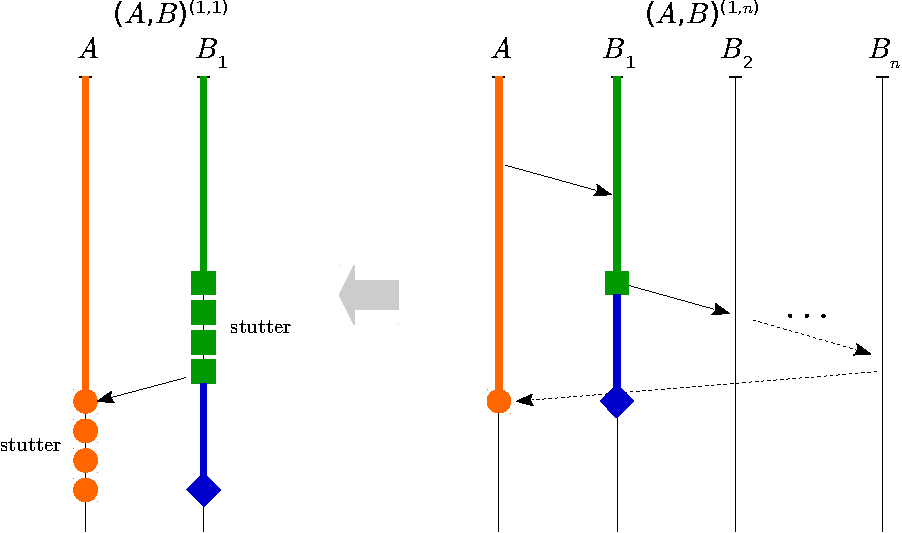
\includegraphics[scale=0.7]{token-systems/figures/simulation_proof}}
      \caption{Constructing a run of a cutoff system from a run of a large system.
        Vertical lines depict (local) paths of the processes,
        the horizontal lines mean the token transmission.
        The process $A$ starts with the token.%
      }
      \label{amba:fig:simulation_proof_1}
    \end{figure}
    We copy the behaviors of processes $A$ and $B_1$ until before $B_1$ sends the token.
    At this moment, we postpone sending the token by $B_1$ and stutter\footnote{
      To ``stutter a process $p$'' means ``not to schedule it''.
      As a result, a stuttered process neither reads inputs nor changes its state.
      In the figures it is shown by repeating a state.%
    }
    it,
    while the process $A$ continues execution until it gets into state \textcolor{orange}{$\CIRCLE$}
    ready to receive the token.
    Then $B_1$ transmits the token to process $A$.
    After that we move process $B_1$ into state \textcolor{blue}{$\blacklozenge$},
    while $A$ stutters in \textcolor{orange}{$\CIRCLE$}.
    Now we are in the original situation and repeat the construction.
    Since the property talks about process $A$ only, the resulting run satisfies it.
    Finally, we assumed that the processes of the large system pass the token infinitely often.
    If some process $B_x \in \{B_1,...,B_n\}$ holds the token forever,
    then we use its behavior for $B_1$ in the cutoff system
    (this may require to insert stuttering steps into behaviors of $B_1$ and $A$ of the cutoff system,
     to synchronize their (finitely many) token transmissions).

    Consider direction $\Leftarrow$. After contra-positioning:
    $$
    (A,B)^{(1,1)} \not\models \varphi(A) ~~\Rightarrow~~ \largesys \not\models \varphi(A).
    $$
    Given a system run of $(A,B)^{(1,n)}$ that satisfies $\neg\varphi(A)$,
    we build a system run of $(A,B)^{(1,1)}$ that satisfies $\neg\varphi(A)$.
    Figure~\ref{amba:fig:simulation_proof_2} shows how to construct a run of a system
    that has one more $B$ process than the cutoff system.
    By repeating the construction we can add the necessary $n-1$ $B$-processes.
    The construction works as follows.
    \begin{figure}[t]\centering{
      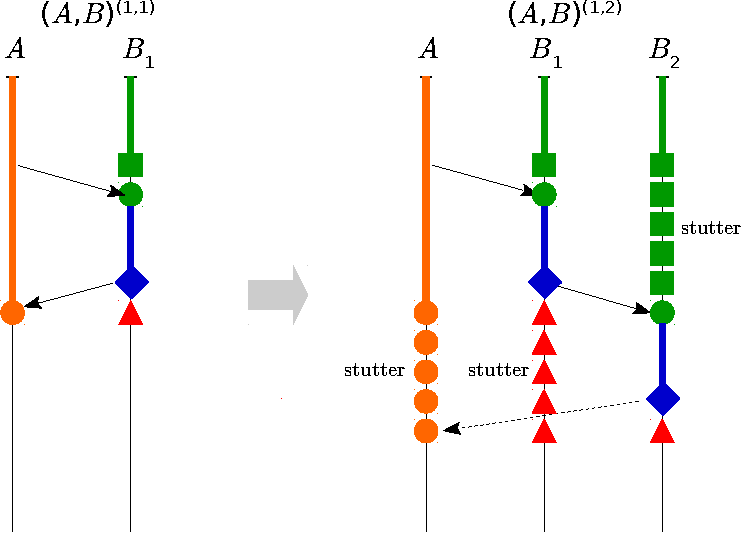
\includegraphics[scale=0.7]{token-systems/figures/simulation_proof2}}
      \caption{Constructing a run of a system $(A,B)^{(1,2)}$ from a run of a cutoff system $(A,B)^{(1,1)}$.
        Vertical lines depict (local) paths of the processes,
        the horizontal lines mean the token transmission.
        The process $A$ starts with the token.%
      }
      \label{amba:fig:simulation_proof_2}
    \end{figure}
    The new process $B_2$ copies the behavior of $B_1$ until before $B_1$ receives the token
    (i.e., up to the state \textcolor{green}{$\rule{0.6em}{0.6em}$}).
    Then it stutters in \textcolor{green}{$\rule{0.6em}{0.6em}$} awaiting for the token from process $B_1$.
    After that it copies $B_1$ behavior from state \textcolor{green}{$\CIRCLE$} till \textcolor{blue}{$\blacklozenge$},
    while processes $A$ and $B_1$ stutter.
    Then $B_2$ sends the token to $A$ and we return to the original situation.
    Finally, the case of $B_1$ or $A$ holding the token forever is straightforward.

    \parbf{Item (2)}
    Consider the case $\forall i. \varphi(B_i)$.
    First, we use the symmetry argument: for every $n$,
    $$
    \largesys \models \forall i.\varphi(B_i) ~\Iff~ \largesys \models \varphi(B_1).
    $$
    It holds because, for every $B_i$ and system run that satisfies $\neg\varphi(B_i)$,
    we can construct a run that satisfies $\neg\varphi(B_1)$.
    The latter is possible because all $B$-processes start without the token and $\varphi$ is 1-indexed%
    \footnote{%
      In contrast,
      the symmetry argument will not work for properties of the form $\forall i. \varphi(A,B_i)$,
      because $B_1$, $B_n$, and $B_{x \in \{2,...,n-1\}}$ have different ``relation'' to $A$.
      For example, take the formula $\forall i. \G(\token_A \impl \token_A \W \token_i)$.
      The (wrongly applied) symmetry argument would produce $\G(\token_A \impl \token_A \W \token_1)$,
      which says that the token moves from $A$ to $B_1$ (trivially true in every system),
      but the original formula does not hold.%
    }.

    After applying the symmetry argument,
    we can use the very same constructions as in item (1),
    see Figures~\ref{amba:fig:simulation_proof_1}~and~\ref{amba:fig:simulation_proof_2}.
    Let us only note the case when the token is stuck in some process.
    As for the construction in Figure~\ref{amba:fig:simulation_proof_2},
    this is simple: the token will be stuck in $A$ or in $B_1$ in the large system too.
    Consider the case in Figure~\ref{amba:fig:simulation_proof_1},
    when the token gets stuck in some process $B_d$ for $d \neq 1$.
    This is the only place in the proof where we use the peculiar structure of the formula to verify:
    $A^B_{loc,1} \land \GF\token_1 \impl \psi(B_1)$.
    Recall that the contra-position negates it and gives 
    $A^B_{loc,1} \land \GF\token_1 \land \neg \psi(B_1)$.
    Thus, in the large system the process $B_1$ receives the token infinitely often,
    and we can simply ignore the case\footnote{%
      We \emph{did} consider the case in other proof branches,
      to avoid relying on the peculiarity of the formula.
      We conjecture that in the case of (more general) properties of the form $\forall i. \varphi(B_i)$ (without $\GF\token_i$),
      the cutoff increases to $(1,2)$.%
    }.
  \end{proof}

  Let us note that without the assumption ``$A$ starts with token'' the constructions break.
  We conjecture that in this case a cutoff increases to $(1,2)$.

\subsection{Experiments} \label{amba:sec:experiments}

  In this section,
  we describe optimizations that are crucial for the synthesis of the parameterized AMBA,
  and present synthesis timings and resulting implementations.
  Most of the optimizations were already described in Section~\ref{tok_rings:sec:optimizations}.
  One interesting and not previously described optimization is ``Decompositional synthesis'',
  where the specification is synthesized incrementally, starting from a subset of the properties.
  It is this optimization that allowed us to synthesize the AMBA.

\parbf{Prototype}
  Our prototype is based on our tool \textsc{Party}~\cite{party},
  a synthesizer of parameterized token rings.
  \textsc{Party} is written in Python,
  uses LTL3BA~\cite{LTL3BA} for automata translation and Z3~\cite{Moura08} for SMT solving.
  The prototype and specification files can be found at \small{\url{https://github.com/5nizza/Party/}} (branch `amba-gr1').
  The experiments were run on a x86\_64 machine with $2.6$GHz CPU, $12$GB RAM, Ubuntu OS.

\parbf{Synchronous hub abstraction (Section~\ref{tok_rings:sec:optimizations})}
  Synchronous hub abstraction can be applied to 1-indexed specifications.
  It lets the environment simulate all but one process, and always schedules this process.
  Thus, the synthesizer searches for a process template in the synchronous setting
  with additional assumptions on the environment, namely: 
  (i) the environment sends the token to the process infinitely often, and
  (ii) the environment never sends the token to the process if it already has it.
  The synchronous hub abstraction is \emph{sound and complete} for 1-indexed properties.
  After applying this optimization \emph{any} monolithic synthesis method
  can be applied to the resulting specification
  (in the form of Eq.\ref{tok_rings:eq:hub-abstraction} on page~\pageref{tok_rings:eq:hub-abstraction}).

\parbf{Hardcoding states with and without the token~\cite[Section4]{Khalimov13}}
  The number of states with and without the token in a process template
  defines the degree of the parallelism in a token ring.
  Parallelism increases with the number of states that do not have the token.
  In the AMBA case study, any grants related action depends on having the token.
  Thus we divide the states in the process template:
  (a) one state does not have the token, while
  (b) all other states have the token.
  We do this by hardcoding the $\tok$ output function.

\parbf{Decompositional synthesis of different grant schemes}
  The idea of the decompositional synthesis is:
  synthesize a subset of the properties,
  then synthesize a larger subset using the model from the previous step as the basis.
  %   As will be noted in the experiments section, all previous optimizations still do not allow us to synthesize AMBA.
  %   It is a successive synthesis approach of properties together with hardcoding token states (next paragraph) that have made it.
  Consider an example of the synthesis of the non-0-process of AMBA.
  The flow is: 
  \begin{enumerate}
  \- Assume that every request is a locked request of type \hburstfour, i.e., 
     add the assumption $\always(\hlocki\land\hburst=\hburstfour)$ to the specification.
     This implicitly removes guarantee G2 and assumption A1 from the specification.
     Synthesize the model. The resulting model has $10$ states (states $t0,..,t9$ and transitions between them in Figure~\ref{amba:fig:ith-model}).

  \- Use the model found in the previous step as the basis:
     assert the number of states, values of output functions in these states, transitions for inputs that satisfy the previous assumption.
     Transitions for inputs that violate the assumption from step 1 are not asserted, and thus are left to be synthesized.

     Now relax the assumptions: allow locked and non-locked \hburstfour\ requests, i.e., replace the previous assumption with $\always(\hburst=\hburstfour)$.
     Again, this implicitly removes G2 and A1.
     In contrast to the last step, now guarantee G3 is not necessarily `activated' if there is a request.

     Synthesize the model.
     This may require increasing the number of states (and it does, in the case of non-0 process)---add new states and keep assertions on all the previous states.

  \- Assert the transitions of the model found, as in the previous step.\\
     Remove all added assumptions and consider the original specification.
     Synthesize the final model.
\end{enumerate}

Although for AMBA this approach was successful, it is not clear how general it is.
For example, it does not work if we start with locked \hburstfour\ and \hready\ always high,
and then try to relax it.
Also, the separation into sets of properties to be synthesized was done manually.

% 
\begin{figure}[t]\centering{
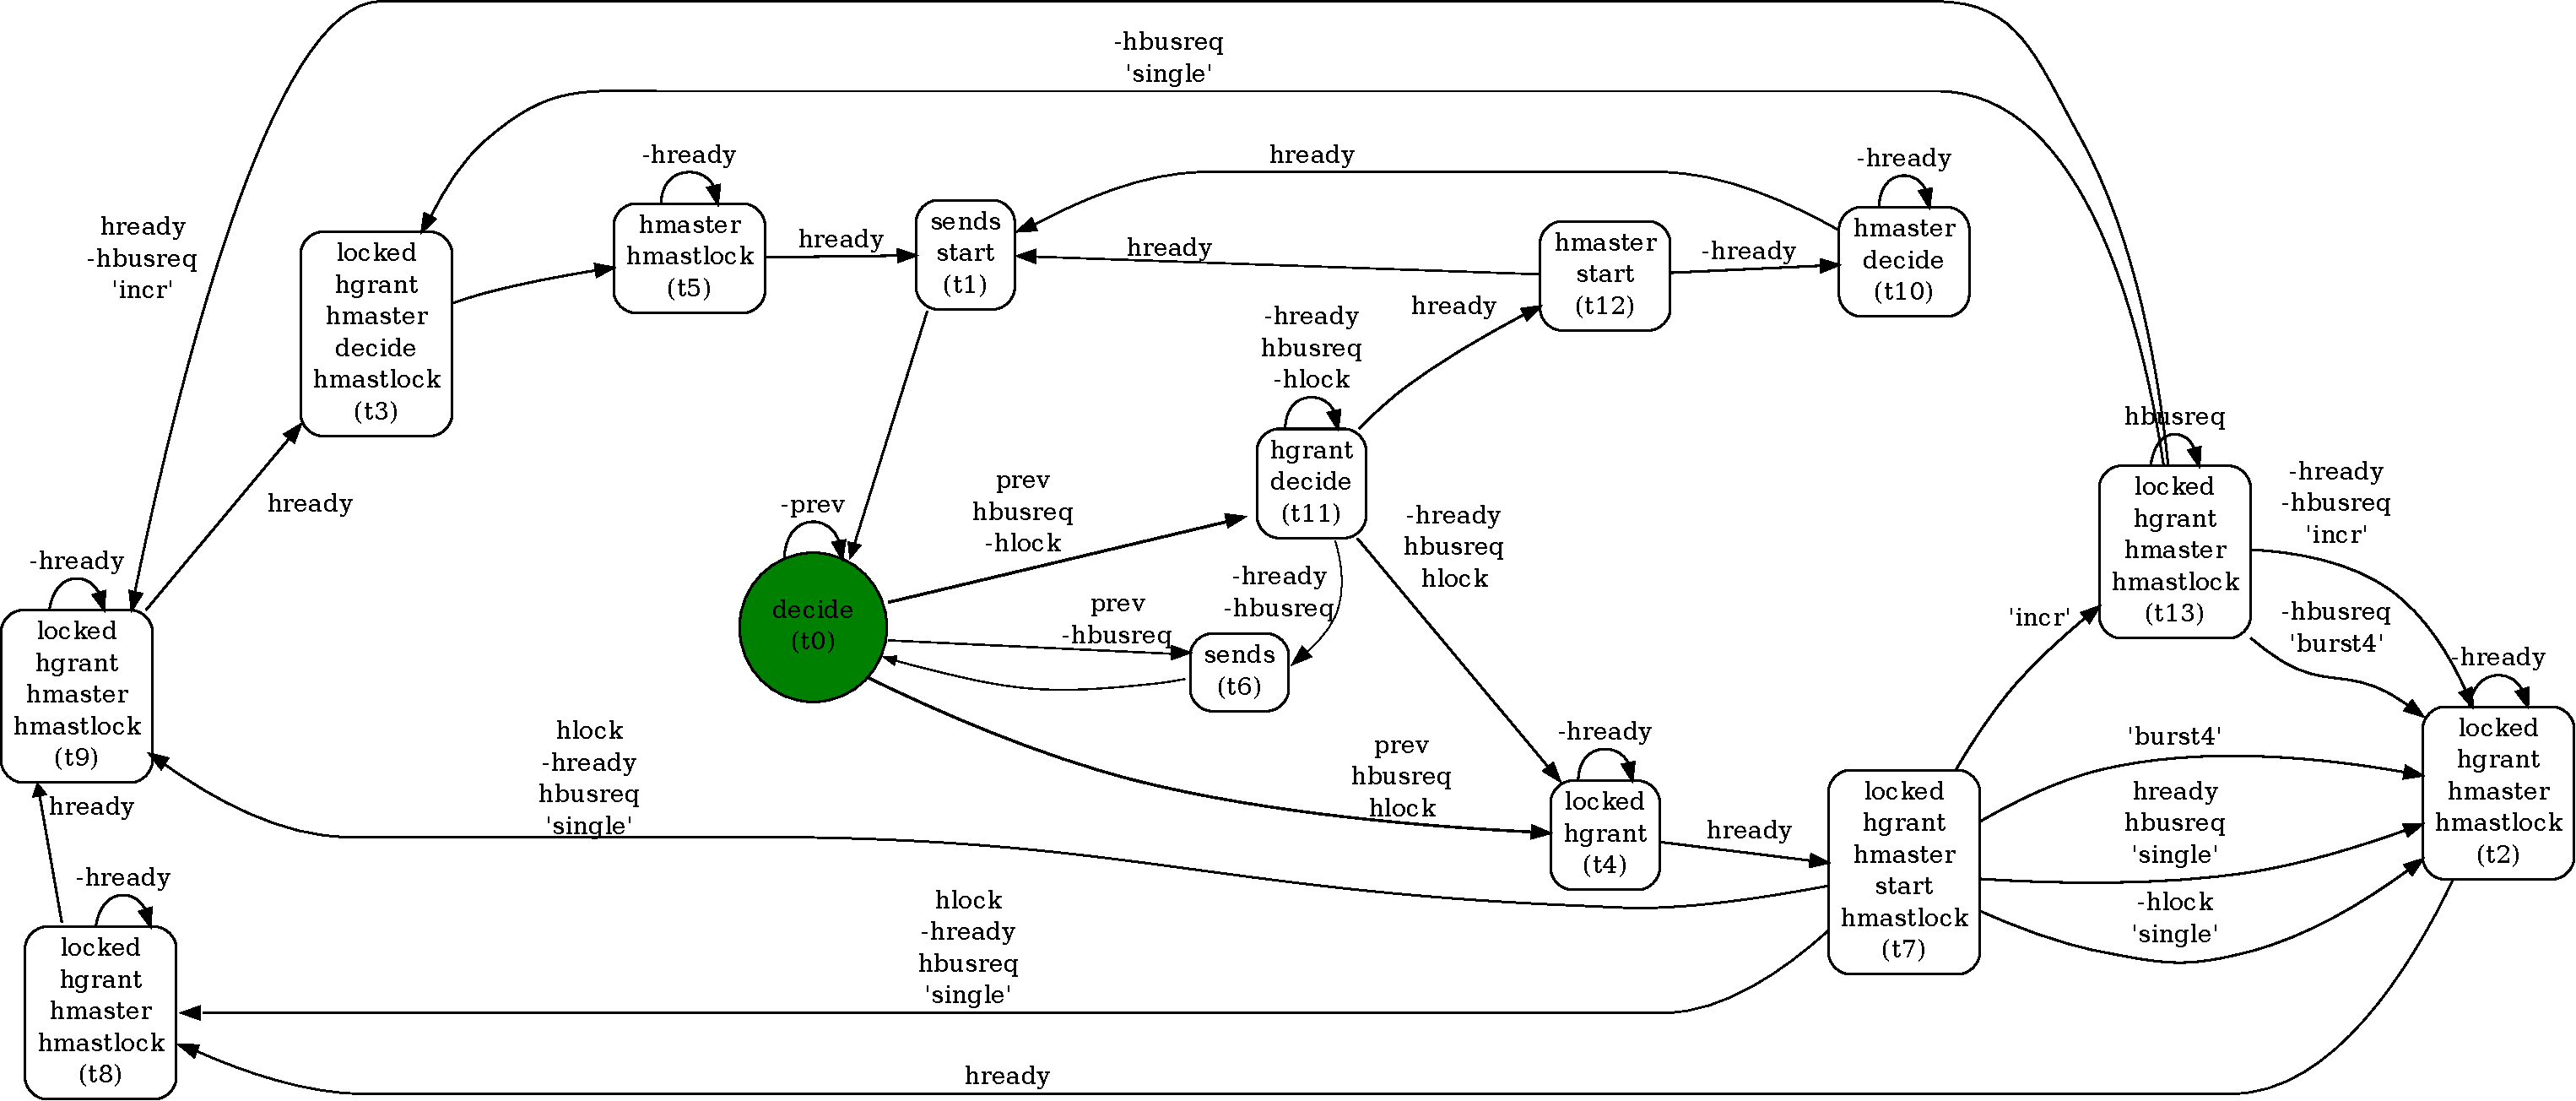
\includegraphics[width=\textwidth]{token-systems/figures/ith-model}}
\caption{Synthesized model of non-$0$-processes (after manual simplification).
Circle green state ($t0$) is without the token, other states are with the token.
The initial state is $t0$.
States are labeled with their active outputs.
Edges are labeled with inputs, a missing input variable means ``don't care''.
`Burst4' means $\hburst=\hburstfour$, `incr' means $\hburst=\hincr$, `single' means neither of them.
In the first step of decompositional synthesis states $t0,..,t9$ were synthesized, in the second $t10,..,t12$ were added, in the final step state $t13$ was added.}
\label{amba:fig:ith-model}
\end{figure}
%
\begin{figure}[t]\centering{
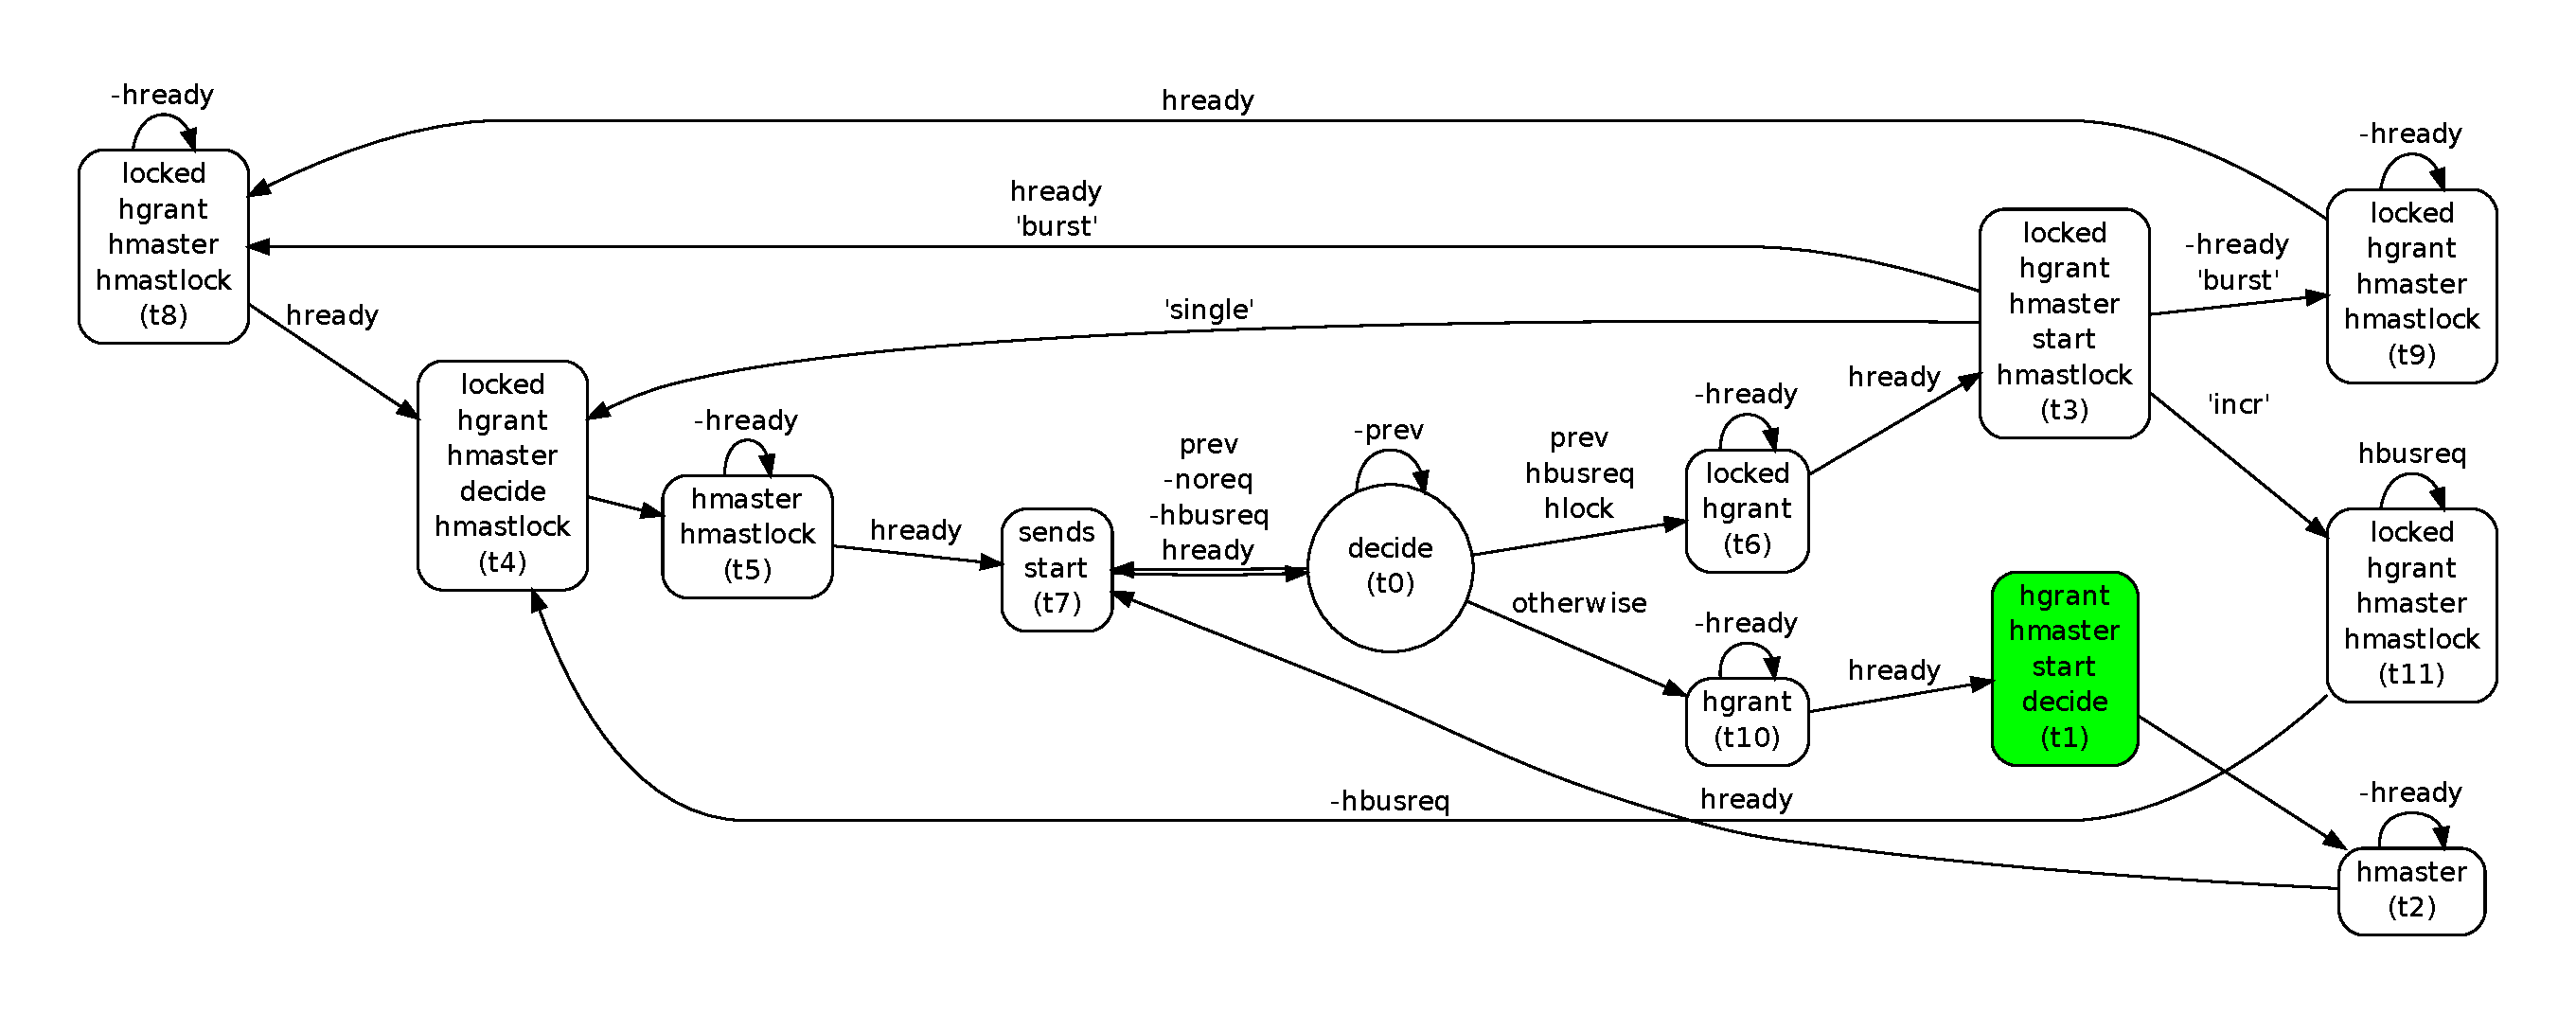
\includegraphics[width=\textwidth]{token-systems/figures/0-model}}
\caption{Synthesized model of $0$-processes (after manual simplification).
Circle state ($t0$) is without the token, other states are with the token.
The initial state is $t1$.
States are labeled with their active outputs.
Edges are labeled with inputs, a missing input variable means ``don't care''.
`Burst' means $\hburst=\hburstthree$ (recall we decreased the length of bursts for 0 process), `incr' means $\hburst=\hincr$, `single' means neither of them.
In the first step of decompositional synthesis states $t0,..,t10$ were synthesized, in the second only transitions were synthesized, but no new states added, in the final step $t11$ was added.}
\label{amba:fig:zero-model}
\end{figure}
%\todo{can we reuse ith models for the zero-process?}


%\parbf{Optimization of SMT Encoding}\label{sec:simpleGR1}
%%
%\newcommand{\Atm}{\ensuremath{{A_{\neg\varphi}}}}
%Recall from Section~\ref{sec:approach} that SMT based bounded synthesis, given an automaton \Atm\ of the negation of specification $\varphi$ and an unknown process template $P=(\Locals_P, \LocalsI, \ActionsProc, \delta_P, out)$ with a fixed number of states, encodes the product automaton $\Atm \times P$ into SMT constraints such that $\Atm \times P$ contains no reachable loops with an accepting state of the \Atm\ iff SMT constraints are satisfiable.
%Below is a general assertion from which the SMT query is composed: 
%$$
%\bigwedge{q\in Q_P}
%\bigwedge{\trans{a}{b}{i,o}\in \delta_\Atm}: \ \ \ 
%\rho(a,q) \ge 0 \land o=out(q) 
%\impl
%\rho(b,\delta_P(q,i)) 
%% 
%% [> \text{ if } b \text { is accepting, else } \ge] 
%\vartriangleright
%\rho(a,q)
%$$
%where $\vartriangleright$ is `$>$' if $b$ is an accepting state of \Atm, else `$\ge$'.
%In words: for any state of the process template, and any transition of the automaton, if the current state of the product automaton is reachable, then the next state should also be reachable and the ranking function should be as stated.
%
%The specification of AMBA we synthesize is derived from GR(1) specification.
%As a consequence it contain assumptions (A3, A6) of the form
%$\always\alpha(i)$ where $\alpha(i)$ is a Boolean formula over current inputs, and many guarantees (G1, G4, G5, G6, G7, G8, G12, G10.2) of the form $\always\beta(i,o,o')$ where $\beta(i,o,o')$ is a Boolean formula over current inputs and outputs and next outputs.
%Instead of using the standard approach via automaton translation described above, we:
%\begin{enumerate}
%  \item encode assertions of the form $\always\alpha(i)$ directly into SMT constraints, namely add $\alpha(i)$ to the the premise of the SMT rule. 
%  Thus, the premise becomes  
%  `$\rho(a,q)\ge 0 \land o=out(q) \mathbf{\land \alpha(i)} \impl ...$'
%
%  \item for all guarantees of the form $\always\beta(i,o,o')$ add SMT constraints of the form: 
%  $$
%  \bigwedge{q \in Q_P} \bigwedge{i \in \ActionsProc}: \ \ 
%  \alpha(i) \impl \beta(i,out(q),out(\delta_P(q,i)))
%  $$
%\end{enumerate}
%The first optimization is sound and complete, the second one: introduces incompleteness if used for model checking (since a given model may have unreachable state that violate the assertion), and seems to be complete for the synthesis.
%
%For AMBA specification in Figure~\ref{amba:fig:AMBAspecNewI} and \ref{amba:fig:AMBAspecNew0} this optimization means that only guarantees G2, G3, G9, G10.1, G11 require the standard flow via automata translation.
%
%Does this optimization help in the synthesis? 
%Preliminary experiments (considering the first step of the decompositional synthesis of non-0 process) show: 
%\begin{itemize}
%\item 
%With the optimization the automaton for the negated specification has 24 states, without -- 42 states.
%
%\item
%The synthesis time with optimization is 16 minutes, without -- 57 minutes.
%Interesting to note that the optimized and non-optimized versions spent the same time (2 minutes) checking satisfiability of the last query (with the model size of 10), so the main difference is in checking unsatisfiable queries -- Z3 identifies unsatisfiability of optimized queries faster (14 vs. 53 minutes).
%A similar behavior happens for a version of the same specification with reduced lengths of bursts ($3/4\impl 2/3$): total times are 3/6 minutes, but the last query took 1m40s/30s for optimized/non-optimized version. 
%
%\end{itemize}


%%%%%%%%%%%%%%%%%%%%%%%%%%%%%%%%%%%%%%%%%%%%%%%%%%%%%%%%%%%%%%%%%%%%%%%%%%%

\parbf{Results}
Synthesis times are in Tables~\ref{amba:tab:non-zero-process}~and~\ref{amba:tab:zero-process}, 
the model synthesized for non-0 process is in Figure~\ref{amba:fig:ith-model}.
The table has timings for the case when all optimizations described in this section are enabled --- it was not our goal to evaluate the optimizations separately, but to find a combination that works for the AMBA case study.

For the $0$-process we considered a simpler version with burst lengths reduced to 2/3 instead of the original 3/4 ticks.
With the original length, the synthesizer could not find a model within 2 hours (it hanged checking 11 state models, while the model has at least 12 states).

Without the decompositional approach,
the synthesizer could not find a model for for non-0 process of the AMBA specification within 5 hours.

\begin{table}[tb]
\footnotesize
\centering
\begin{minipage}[b]{0.45\textwidth}
\centering
% \setlength{\tabcolsep}{4pt}
\begin{tabular}{ l|cc }
Addit.\ assumptions                          & time & \#states \\
\hline
\rule{0pt}{3ex} \specialcellC{$\always \hlock$ \\ $\always \hburst=\hburstfour$} 
                       & 16min.  & 10  \\
\hline
\rule{0pt}{2ex} \specialcellC{$\always \hburst=\hburstfour$} & 13sec.  & 13  \\
\hline
\rule{0pt}{2ex} 
-- (Full Specification) & 1min.  & 14 \\
\end{tabular}
\caption{Results for non-$0$ process.\\~}
\label{amba:tab:non-zero-process}
\end{minipage}
% 
\hspace{0.5cm}
% 
\begin{minipage}[b]{0.45\textwidth}
\centering
% \setlength{\tabcolsep}{4pt}
\begin{tabular}{ l|cc }
Addit. assumptions & time & \#states \\
\hline
\rule{0pt}{3ex} \specialcellC{$\always \hlock$ \\ $\always \hburst=\hburstfour$} 
                       & 3h.  & 11  \\
\hline
\rule{0pt}{2ex} \specialcellC{$\always \hburst=\hburstfour$} & 1min.  & 11  \\
\hline
\rule{0pt}{2ex} 
-- (Full Specification) & 1m30s.  & 12 \\
\end{tabular}
\caption{Results for $0$-process \\ (bursts reduced: $3/4 \rightarrow 2/3$).}
\label{amba:tab:zero-process}
\end{minipage}
\end{table}

%\ak{`decide' is not faithfully simulated in token passing simulations?}


\subsection{Discussion}

We have shown that parameterized synthesis in token rings can be used to 
solve benchmark problems of significant size, in particular the well-known 
AMBA AHB specification that has been used as a synthesis benchmark for a long 
time. To achieve this goal, we slightly extended the cutoff results that 
parameterized synthesis is based on, and used a number of optimizations in 
the translation of the specification and the synthesis procedure itself to 
make the process feasible.

This is the first time that the AMBA case study, or any other realistic case,
has been solved by an automatic synthesis 
procedure for the parameterized case. However, some of the steps in the 
procedure are manual or use an ad-hoc solution for the specific problem at 
hand, like the limited extension of cutoff results for global inputs, the 
construction of suitable functions to convert local to global outputs, or the 
decompositional synthesis for different grant schemes. Generalizing and 
automating these approaches is a possible future work.

Our synthesized implementation is such 
that the size of the parallel composition grows only linearly with the number of 
components. Thus, for this case study our approach does not only solve the 
problem of increasing synthesis time for a growing number of components, but 
also the problem of implementations that need an exponential amount of memory 
in the number of components. We pay for this small amount of memory with a 
less-than-optimal reaction time, as processes have to wait for the token in 
order to grant a request. This restriction could be remedied by extending the 
parameterized synthesis approach to different system models, e.g., processes 
that coordinate by guarded transitions~\cite{EmersonK03},
or communicate via broadcast messages~\cite{EsparzaFM99}.
